\documentclass[11pt,a4paper]{article}
\usepackage[T1]{fontenc}
\usepackage[margin=1in]{geometry}
\usepackage{amsmath,amssymb,booktabs,array}
\usepackage{pgfplots,lmodern,microtype,caption,placeins,graphicx,pdflscape,iftex}
\ifLuaTeX\usepackage{luacode}\fi
\graphicspath{{assets/}{}}
\captionsetup{font=small,labelfont=bf}
\definecolor{scblue}{HTML}{0072B2}
\definecolor{storange}{HTML}{D55E00}
\usepackage{hyperref}
\pgfplotsset{compat=1.18,every axis/.append style={
axis line style={gray!60},tick style={gray!60},grid style={gray!15},
legend style={draw=none,font=\small},label style={font=\small},tick label style={font=\small}}}
\hypersetup{colorlinks=true,linkcolor=black,urlcolor=blue,citecolor=black}
\setlength{\parindent}{0pt}
\setlength{\parskip}{0.55em}
\renewcommand{\arraystretch}{1.12}
\title{Caste Composition and Rural Electrification in India:\\An Exploratory Regression-Discontinuity Extension}
\author{nakshatra0904}
\date{12 October 2026}
\raggedbottom
\makeatletter
\setlength{\@fptop}{0pt}
\setlength{\@fpsep}{18pt}
\setlength{\@fpbot}{0pt plus 1fil}
\makeatother
\ifLuaTeX
\begin{luacode*}
local figures = {"01_population_frequencies.pdf",
"02_baseline_caste_distributions.pdf",
"03_caste_composition_balance.pdf",
"04_rd_vd_pwr_d_dom_11.pdf",
"05_rd_hpca11_msl_elec.pdf",
"06_rd_hpca01_msl_elec.pdf",
"07_access_and_adoption_by_group.pdf",
"08_primary_caste_heterogeneity.pdf",
"09_employment_heterogeneity.pdf",
"10_bandwidth_sensitivity.pdf",
"11_specification_sensitivity.pdf",
"12_baseline_balance.pdf",
"13_majority_group_rdd.pdf",
"14_state_sample_coverage.pdf",
"15_pre_policy_nightlight_checks.pdf",
"16_access_adoption_gap.pdf",
"17_productive_electricity_rdd.pdf",
"18_productive_electricity_heterogeneity.pdf"}
local alphabet = "ABCDEFGHIJKLMNOPQRSTUVWXYZabcdefghijklmnopqrstuvwxyz0123456789+/"
local lookup = {}
for i=1,#alphabet do lookup[alphabet:sub(i,i)] = i-1 end
local function decode(data)
  local result, value, bits = {}, 0, 0
  for char in data:gmatch(".") do
    local digit = lookup[char]
    if digit then
      value = (value << 6) | digit
      bits = bits + 6
      if bits >= 8 then
        bits = bits - 8
        result[#result+1] = string.char((value >> bits) & 255)
        value = value & ((1 << bits) - 1)
      end
    end
  end
  return table.concat(result)
end
for _,name in ipairs(figures) do
  local localfile = io.open("assets/"..name,"rb") or io.open(name,"rb")
  if localfile then localfile:close()
  else
    local encoded = assert(io.open(name..".b64","r"),"Missing figure input: "..name)
    local data = encoded:read("*a"); encoded:close()
    local output = assert(io.open(name,"wb")); output:write(decode(data)); output:close()
  end
end
\end{luacode*}
\fi
\begin{document}
\maketitle
\begin{abstract}
I examine whether eligibility for India's Rajiv Gandhi Grameen Vidyutikaran Yojana (RGGVY) generated different local electricity-access and household-adoption gains in villages with different pre-policy Scheduled Caste (SC) and Scheduled Tribe (ST) population shares. I extend the public replication data and population-threshold design of Burlig and Preonas (2024), using a 300-person eligibility boundary and a local sample of 12,533 villages. Local-linear models include separate caste-share and population-slope interactions, state effects, triangular weights and block-clustered inference. I find no clear evidence of effect heterogeneity in the four primary tests after Holm correction. A ten-percentage-point higher SC share is associated with a -0.76-percentage-point difference in the household-lighting eligibility effect, with a 95\% interval of [-1.56, +0.04]; the corresponding ST difference is -0.39. Descriptive social gaps remain substantial, but they do not establish unequal causal gains from this policy rule. Commercial-access and employment analyses are explicitly exploratory. This is a replication-based analytical extension, not a claim to be the first study of caste and electricity.
\end{abstract}

\section{Introduction and research contribution}
Extending the grid to a settlement does not guarantee household adoption or reliable supply. These are distinct margins of electricity access. I ask whether an eligibility rule produced comparable gains across villages with different baseline SC and ST composition, while keeping the two social categories separate.

My contribution is a narrowly defined test of heterogeneity in the local policy-induced discontinuity. I do not identify the causal effect of caste identity or discrimination, or individual SC/ST household treatment effects. I have not established publication-level novelty.

\section{Related literature and policy setting}
Burlig and Preonas \cite{burlig} evaluate RGGVY using regression discontinuity and difference-in-differences. Their clearest village-level access gains occur in commercial and all-sector electricity; domestic access was already widespread near the eligibility threshold. Sedai and coauthors \cite{sedai} examine marginalized households' access, reliability and welfare using IHDS panel data and instrumental variables. Dugoua and coauthors \cite{dugoua} study geographic and socioeconomic barriers. Azam \cite{azam} studies later village-level reliability and tribal concentration. The broad social-inequality question is therefore already established; I address heterogeneity in a specific early policy-assignment mechanism.

For the relevant first-wave regime, eligibility depended on 2001 Census population being at least 300. The policy rule applied to habitations. Following the underlying study, I use single-habitation villages so that Census village population corresponds to the assignment unit. Later 100-person eligibility rules are not combined with the 300-person design.

\section{Data, measurement and sample construction}
The real source file contains 580,643 records and 943 variables. I verified its 2,294,890,843-byte size and MD5 checksum against the public Dataverse archive \cite{data}. The delivered compact extract contains 55,320 candidate villages and only documented analysis columns. I checked identifier uniqueness and the ranges of shares and binary outcomes. I used no synthetic observations.

\begin{table}[htbp]\centering
\caption{Sample construction}
\label{tab:sample}
\begin{tabular}{p{0.72\linewidth}r}\toprule
Selection stage & Villages \\ \midrule
Source archive & 580,643 \\
First wave and valid geography & 172,076 \\
Matched, single habitation, positive population; Kerala excluded & 79,724 \\
Candidate extract: population 1--999 & 55,320 \\
Preferred sample: population 100--499 & 24,422 \\
Main sample: population 200--399 & 12,533 \\
\bottomrule\end{tabular}
\end{table}

I constructed the preferred sample using the authors' first-wave, geography, night-light and habitation-match flags. Kerala is excluded following the original code. It also excludes Census/habitation population mismatches exceeding 20\% and projected night-light changes of at least 20 units. A sensitivity retains observations excluded by the post-policy light-change filter. The main sample spans 12 states, 129 districts and 1,342 blocks. Exact source flags and exclusions are recorded in the data dictionary and sample-flow CSV.

Primary outcomes are 2011 domestic village electricity availability, a binary Census indicator, and the village share of households using electricity as their main lighting source. Neither measure is kWh or continuous supply reliability. Moderators are \emph{2001} SC and ST population shares. Employment outcomes are village work-participation shares; female participation uses the female-population denominator. ``Other work'' excludes agriculture and household industry.

\section{Empirical strategy}
Let $P_i$ denote village $i$'s 2001 population, $x_i=P_i-299.5$, and $D_i=\mathbf{1}\{P_i\geq300\}$. The half-person cutoff represents the assignment boundary for integer population. Define $G_{ig}$ as the baseline population share of group $g$, divided by $0.1$, for $g\in\{SC,ST\}$. Within a bandwidth $h$, I estimate
\begin{align}
Y_i ={}& \alpha_{s(i)}+\tau D_i+\beta_-x_i+\beta_+D_ix_i \nonumber\\
&+\sum_{g\in\{SC,ST\}}\left(\theta_gG_{ig}+\delta_gD_iG_{ig}
+\lambda_gx_iG_{ig}+\kappa_gD_ix_iG_{ig}\right)+\varepsilon_i.
\label{eq:main}
\end{align}
Here $\alpha_{s(i)}$ are state fixed effects. Both caste-specific population slopes and their side-specific interactions are included. Thus $\delta_g$ measures how the eligibility effect changes with a ten-percentage-point increase in baseline group share. It does not identify a causal effect of group composition itself.

The main bandwidth is $h=100$ persons; observations receive triangular weights $w_i=1-|x_i|/h$. Standard errors use block-clustered CR1 covariance and cluster-based $t$ inference. Sensitivities use bandwidths of 50, 150 and 200, district clustering, a five-person donut, baseline adjustment and state-specific discontinuities and slopes. The widest local window remains below the distinct 500-person road-policy boundary.

The estimand is a local \emph{intent-to-treat} effect of eligibility. Continuity of potential outcomes and moderator-specific response surfaces at the boundary is required. Integer population and heaping warrant caution. Fixed-bandwidth heterogeneity intervals are conventional and exploratory; they do not correct smoothing bias. Pooled benchmarks use \texttt{rdrobust} with robust bias-corrected intervals and mass-point adjustment \cite{rdrobust}. No domestic-electricity fuzzy-RDD local average treatment effect is claimed because the primary domestic-access first stage is weak.

I treat the four primary caste-interaction tests as one Holm-adjusted family and the twelve secondary tests as a separate exploratory family. I added commercial and all-sector availability after examining the first primary benchmark and the original paper's Table~2. They were not retrospectively designated primary outcomes; the dated analysis plan records this amendment.

\section{Results}
\subsection{Pooled regression-discontinuity benchmarks}
Table~\ref{tab:pooled} reports the policy-eligibility jump before asking whether it varies with caste composition. The pooled model adjusts for state covariates and uses local-linear point estimation, local-quadratic bias correction and block-clustered CR1 inference. Its robust intervals use the package's normal approximation. Data-driven bandwidths are MSE-optimal; fixed benchmarks use $h=100$ and $b=150$. The 100--499-person input window avoids the distinct 500-person road threshold.

\begin{table}[htbp]\centering\footnotesize
\setlength{\tabcolsep}{4pt}
\caption{Pooled RDD: bias-corrected eligibility effects}
\label{tab:pooled}
\begin{tabular}{@{}llrrrr@{}}\toprule
Outcome & Bandwidth & Effect (pp) & Robust 95\% interval & $p$ & $N_h$\\\midrule
Domestic availability & MSE & -0.72 & [-3.76, +2.33] & 0.645 & 7,533 \\
Domestic availability & $h=100$ & -0.54 & [-2.93, +1.85] & 0.657 & 12,529 \\
Household lighting & MSE & +1.09 & [-2.23, +4.41] & 0.521 & 10,682 \\
Household lighting & $h=100$ & +1.10 & [-1.94, +4.14] & 0.479 & 12,533 \\
Commercial availability & MSE & +3.59 & [-1.74, +8.91] & 0.187 & 8,666 \\
Commercial availability & $h=100$ & +3.67 & [-0.82, +8.16] & 0.110 & 12,529 \\
All-sector availability & MSE & +2.86 & [-2.61, +8.33] & 0.306 & 8,267 \\
All-sector availability & $h=100$ & +2.94 & [-1.60, +7.49] & 0.204 & 12,529 \\
\bottomrule\end{tabular}
\par\smallskip\raggedright
Notes: $N_h$ is the number of villages in the estimation bandwidth, rather than the full input or bias-correction window. Fixed-$h$ models contain 1,342 blocks in the estimation window and 1,454 in the bias-correction window. All intervals include zero. These benchmarks differ from the original paper's preferred controls and variance specification and are not an exact replication of its tables. Unadjusted benchmark $p$-values are descriptive and do not replace the four-test primary heterogeneity family. Complete bandwidths, counts and conventional estimates appear in \nolinkurl{tables/pooled_rdrobust.csv}.
\end{table}
\FloatBarrier

\subsection{Primary caste heterogeneity}
\begin{table}[htbp]\centering\small
\caption{Primary effect differences at the eligibility boundary}
\label{tab:primary}
\begin{tabular}{llrrr}\toprule
Outcome & Share & Difference & 95\% interval & Holm $p$ \\ \midrule
Domestic availability & SC & +0.14 & [-0.54, +0.81] & 1.000 \\
Domestic availability & ST & -0.08 & [-0.62, +0.47] & 1.000 \\
Household lighting & SC & -0.76 & [-1.56, +0.04] & 0.257 \\
Household lighting & ST & -0.39 & [-1.09, +0.31] & 0.823 \\
\bottomrule\end{tabular}
\par\smallskip\footnotesize\raggedright
Notes: Differences are percentage points per ten-percentage-point higher baseline share. $h=100$, triangular weights, state effects and block-clustered $t$ intervals. Domestic availability uses 12,529 observations; household lighting uses 12,533.
\end{table}

All four primary adjusted $p$-values exceed 0.05. Household-lighting heterogeneity is estimated at -0.76 pp for SC share (raw $p=0.064$, Holm $p=0.257$) and -0.39 pp for ST share (Holm $p=0.823$). These estimates and intervals do not demonstrate equivalence. Figure~\ref{fig:forest} presents all four tests; Figure~\ref{fig:rdd} shows the unadjusted household-lighting discontinuity for visual context.

\begin{figure}[htbp]\centering
\begin{tikzpicture}
\begin{axis}[width=0.88\linewidth,height=6cm,xlabel={Effect difference (pp per +10 pp baseline share)},
ytick={1,2,3,4},yticklabels={Lighting / ST,Lighting / SC,Domestic / ST,Domestic / SC},
ymin=0.5,ymax=4.5,xmin=-1.8,xmax=1.0,xmajorgrids,axis lines=left,
tick label style={font=\small},label style={font=\small}]
\addplot[black,dashed,no marks,forget plot] coordinates {(0,0.5) (0,4.5)};
\addplot[scblue,only marks,mark=*,mark size=2.5pt,error bars/.cd,x dir=both,x explicit] coordinates {
(0.137046,4) += (0.675583,0) -= (0.675583,0)
(-0.757215,2) += (0.801731,0) -= (0.801731,0)
};
\addplot[storange,only marks,mark=square*,mark size=2.5pt,error bars/.cd,x dir=both,x explicit] coordinates {
(-0.076565,3) += (0.548115,0) -= (0.548115,0)
(-0.388683,1) += (0.697268,0) -= (0.697268,0)
};
\end{axis}\end{tikzpicture}
\caption{Primary caste-interaction estimates and conventional 95\% block-clustered intervals. Source: executed local-linear models using 2001 composition and 2011 outcomes.}
\label{fig:forest}
\end{figure}

\begin{figure}[htbp]\centering
\begin{tikzpicture}
\begin{axis}[width=0.88\linewidth,height=6cm,xlabel={2001 Census population (persons)},
ylabel={Households using electric lighting (\%)},xmin=100,xmax=499,
legend pos=south east,axis lines=left,tick label style={font=\small},label style={font=\small}]
\addplot[scblue,only marks,mark=*] coordinates {(109.748,44.18998) (129.512,46.96079) (149.586,48.27684) (169.299,52.10303) (189.466,53.69364) (209.214,54.88668) (229.250,54.05968) (249.569,55.70299) (269.529,53.98285) (289.499,55.72216)};
\addlegendentry{Below threshold}
\addplot[storange,only marks,mark=*] coordinates {(309.329,57.71018) (329.545,56.66929) (349.439,57.49612) (369.339,58.00922) (389.422,57.54534) (409.615,57.05955) (429.668,55.91140) (449.461,57.76247) (469.512,56.49391) (489.582,57.71088)};
\addlegendentry{Eligible}
\addplot[scblue,no marks] coordinates {(200.00,54.896495) (202.03,54.899973) (204.06,54.903452) (206.09,54.906930) (208.12,54.910408) (210.15,54.913887) (212.18,54.917365) (214.21,54.920844) (216.24,54.924322) (218.28,54.927800) (220.31,54.931279) (222.34,54.934757) (224.37,54.938236) (226.40,54.941714) (228.43,54.945192) (230.46,54.948671) (232.49,54.952149) (234.52,54.955627) (236.55,54.959106) (238.58,54.962584) (240.61,54.966063) (242.64,54.969541) (244.67,54.973019) (246.70,54.976498) (248.73,54.979976) (250.77,54.983455) (252.80,54.986933) (254.83,54.990411) (256.86,54.993890) (258.89,54.997368) (260.92,55.000847) (262.95,55.004325) (264.98,55.007803) (267.01,55.011282) (269.04,55.014760) (271.07,55.018238) (273.10,55.021717) (275.13,55.025195) (277.16,55.028674) (279.19,55.032152) (281.22,55.035630) (283.26,55.039109) (285.29,55.042587) (287.32,55.046066) (289.35,55.049544) (291.38,55.053022) (293.41,55.056501) (295.44,55.059979) (297.47,55.063458) (299.50,55.066936)};
\addplot[storange,no marks] coordinates {(299.50,57.195460) (301.53,57.209859) (303.56,57.224259) (305.59,57.238659) (307.62,57.253059) (309.65,57.267459) (311.68,57.281858) (313.71,57.296258) (315.74,57.310658) (317.78,57.325058) (319.81,57.339457) (321.84,57.353857) (323.87,57.368257) (325.90,57.382657) (327.93,57.397057) (329.96,57.411456) (331.99,57.425856) (334.02,57.440256) (336.05,57.454656) (338.08,57.469055) (340.11,57.483455) (342.14,57.497855) (344.17,57.512255) (346.20,57.526655) (348.23,57.541054) (350.27,57.555454) (352.30,57.569854) (354.33,57.584254) (356.36,57.598653) (358.39,57.613053) (360.42,57.627453) (362.45,57.641853) (364.48,57.656253) (366.51,57.670652) (368.54,57.685052) (370.57,57.699452) (372.60,57.713852) (374.63,57.728252) (376.66,57.742651) (378.69,57.757051) (380.72,57.771451) (382.76,57.785851) (384.79,57.800250) (386.82,57.814650) (388.85,57.829050) (390.88,57.843450) (392.91,57.857850) (394.94,57.872249) (396.97,57.886649) (399.00,57.901049)};
\draw[dashed] (axis cs:299.5,44) -- (axis cs:299.5,60);
\end{axis}\end{tikzpicture}
\caption{Household electric-lighting share in 2011. Dots are 20-person-bin means plotted at mean population; lines are unadjusted triangular local-linear fits within 100 persons. Display lines are extended to the cutoff; formal models include state effects. Source: public RGGVY replication data.}
\label{fig:rdd}
\end{figure}

Descriptively, lighting adoption is lower in SC-majority and ST-majority villages than in other villages in the local sample. Such level differences are not causal policy effects. Domestic village availability was already widespread; its weak local eligibility jump is consistent with the published study. The null primary results do not imply that RGGVY had no effects nationally or on other electricity margins.

\subsection{Exploratory productive-electricity and employment outcomes}
\begin{table}[htbp]\centering\small
\caption{Exploratory caste-interaction results}
\label{tab:secondary}
\begin{tabular}{llrrr}\toprule
Outcome & Share & Difference & 95\% interval & Holm $p$ \\ \midrule
All work & SC & +0.13 & [-0.24, +0.50] & 1.000 \\
All work & ST & +0.06 & [-0.22, +0.35] & 1.000 \\
Female work & SC & +0.09 & [-0.52, +0.70] & 1.000 \\
Female work & ST & -0.04 & [-0.50, +0.42] & 1.000 \\
Other work & SC & +0.06 & [-0.23, +0.36] & 1.000 \\
Other work & ST & +0.02 & [-0.18, +0.22] & 1.000 \\
Female other work & SC & +0.06 & [-0.22, +0.35] & 1.000 \\
Female other work & ST & +0.08 & [-0.12, +0.28] & 1.000 \\
Commercial availability & SC & -1.31 & [-2.67, +0.06] & 0.660 \\
Commercial availability & ST & -0.07 & [-1.08, +0.94] & 1.000 \\
All-sector availability & SC & -1.37 & [-2.71, -0.04] & 0.524 \\
All-sector availability & ST & -0.25 & [-1.24, +0.73] & 1.000 \\
\bottomrule\end{tabular}
\par\smallskip\footnotesize\raggedright
Notes: Same units and main regression design as Table~\ref{tab:primary}. Holm correction covers twelve secondary tests. Commercial/all-sector access was added transparently after the first primary benchmark. No isolated unadjusted result is treated as confirmatory.
\end{table}

The SC interaction for all-sector availability has an unadjusted $p$-value below 0.05, but does not survive the secondary-family correction. Results must therefore not be selected using the most favorable outcome or bandwidth. Complete coefficient tables, joint tests and pooled bias-corrected benchmarks are retained in the repository. Pooled commercial and all-sector point estimates are positive, but their clustered robust intervals include zero under the benchmark used here. This differs from exact replication of the paper's preferred covariate and variance specifications.

\section{Diagnostics and robustness}
Six baseline checks---SC share, ST share, domestic access, household lighting, literacy and 2001 night lights---do not reject after Holm adjustment. This supports, but cannot prove, continuity. Integer-population frequencies and pre-policy annual light discontinuities (1998--2004) are reported separately. No continuous-density diagnostic is presented as proof of no sorting.

\begin{figure}[htbp]\centering
\begin{tikzpicture}
\begin{axis}[width=0.88\linewidth,height=6cm,xlabel={Bandwidth on each side (persons)},
ylabel={Lighting-effect difference (pp per +10 pp share)},xtick={50,100,150,200},
xmin=40,xmax=210,legend pos=south east,axis lines=left,
tick label style={font=\small},label style={font=\small}]
\addplot[black,dashed,no marks,forget plot] coordinates {(40,0) (210,0)};
\addplot[scblue,mark=*,error bars/.cd,y dir=both,y explicit] coordinates {
(50,-0.835579) += (0,1.155081) -= (0,1.155081)
(100,-0.757215) += (0,0.801731) -= (0,0.801731)
(150,-0.583010) += (0,0.668517) -= (0,0.668517)
(200,-0.360009) += (0,0.591049) -= (0,0.591049)
};\addlegendentry{SC}
\addplot[storange,mark=square*,error bars/.cd,y dir=both,y explicit] coordinates {
(50,-0.018102) += (0,0.995561) -= (0,0.995561)
(100,-0.388683) += (0,0.697268) -= (0,0.697268)
(150,-0.207635) += (0,0.579289) -= (0,0.579289)
(200,0.001198) += (0,0.514544) -= (0,0.514544)
};\addlegendentry{ST}
\end{axis}\end{tikzpicture}
\caption{Household-lighting heterogeneity across bandwidths. Intervals use conventional block-clustered inference. Wider windows alter both precision and smoothing bias. Source: executed models.}
\label{fig:bandwidth}
\end{figure}

State-specific discontinuities and slopes produce household-lighting interactions of -0.76 pp for SC share and -0.51 pp for ST share. Other retained specifications remove the post-policy light-change filter, cluster by district, omit observations within five persons of the boundary or adjust for baseline outcomes. Majority-group regressions require at least 50 observations and 20 blocks per side. Placebo cutoffs at 149.5 and 449.5 use 50-person windows that exclude the true boundary. Non-rejection in these exercises cannot establish design validity.

\section{Limitations and policy interpretation}
The estimates apply to small, single-habitation villages near an early policy boundary. They are neither national average effects nor evidence about present-day electricity conditions. Composition is correlated with geography, remoteness and institutions. State-specific response checks help assess geographic confounding but cannot identify a causal effect of caste or discrimination.

Village availability, household adoption and supply reliability must not be conflated. These data cannot establish individual SC/ST household benefits, measured consumption in kWh or continuous service quality. A statistically insignificant effect difference does not establish equal benefits; conventional heterogeneity intervals also leave smoothing-bias concerns.

The defensible policy conclusion is a distinction between disparities and causal responses: descriptive social gaps do not automatically demonstrate unequal gains from this particular eligibility rule. A stronger next study would combine individual caste-specific access and reliability records with later-period outcomes and credible policy assignment. This report is an exploratory, reproducible extension; it is not publication-ready causal evidence of exclusion.

\section{Reproduction and execution status}
I executed the complete R pipeline for data preparation, descriptive statistics, RDD estimation, multiplicity adjustment, robustness and all eighteen graph designs. The reconstructed data and 21 numerical tables reproduce the original reference results within the recorded tolerances. I independently checked all eight main coefficient vectors and CR1 cluster covariance matrices using weighted normal equations and explicit cluster score sums. I also verified the R extract rebuild against the complete original source archive.

Run \texttt{Rscript R/install\_packages.R}, then \texttt{Rscript R/00\_master.R} from the repository root. The master uses the verified source extract and writes to \nolinkurl{r_generated/}. I used R 4.5.1, haven 2.5.5, jsonlite 2.0.0 and rdrobust 4.1.1. Logs, versions, session information and numerical comparisons are retained in \nolinkurl{verification/}. The publication figures and tables, originally produced with Python, are retained as verified reference outputs; the supplied analysis code is now R. The R graphs reproduce the same metrics and designs with native R styling.

The main-text tables and three summary figures are embedded in the source. The complete graphical appendix uses eighteen vector PDF assets in the report folder; compile with that assets folder alongside the source. No external bibliography file is required. The full multi-gigabyte source and published papers are linked rather than bundled. The source archive declares CC0 1.0; the new analysis code is MIT licensed.

\FloatBarrier
\begin{thebibliography}{9}
\bibitem{burlig} Burlig, F., and L. Preonas (2024).
Out of the Darkness and into the Light? Development Effects of Rural Electrification.
\emph{Journal of Political Economy}, 132(9), 2937--2971.
\url{https://doi.org/10.1086/730204}.
\bibitem{data} Burlig, F., and L. Preonas. Public replication archive.
Harvard Dataverse. \url{https://doi.org/10.7910/DVN/APWICK}.
\bibitem{sedai} Sedai, A. K., T. Jamasb, R. Nepal, and R. Miller (2021).
Electrification and welfare for the marginalized: Evidence from India.
\emph{Energy Economics}, 102.
\url{https://www.sciencedirect.com/science/article/abs/pii/S0140988321003595}.
\bibitem{dugoua} Dugoua, E., R. Liu, and J. Urpelainen (2017).
Geographic and socio-economic barriers to rural electrification: New evidence from Indian villages.
\emph{Energy Policy}, 106, 278--287.
\url{https://www.sciencedirect.com/science/article/abs/pii/S0301421517301921}.
\bibitem{azam} Azam, M. (2026).
The Enclave Penalty: Tribes, Caste, and Electricity Reliability in India.
IZA Discussion Paper 18493. \url{https://docs.iza.org/dp18493.pdf}.
\bibitem{rdrobust} Calonico, Cattaneo, Farrell, and Titiunik.
\texttt{rdrobust}: software and methodological references.
\url{https://github.com/rdpackages/rdrobust}.
\end{thebibliography}
\clearpage
\appendix
\section{Regression coefficients and file guide}
\begin{table}[htbp]\centering\small
\caption{Main local-linear interacted regressions}
\label{tab:coefficients}
\begin{tabular}{lrr}\toprule
Regressor & Domestic availability & Household lighting\\\midrule
$D$ & -0.5788 (1.2054) & +3.2153 (1.5911) \\
$x$ & +0.0101 (0.0201) & -0.0293 (0.0253) \\
$D x$ & +0.0016 (0.0284) & -0.0073 (0.0314) \\
$G_{SC}$ & -0.2883 (0.2781) & -0.5691 (0.3199) \\
$D G_{SC}$ & +0.1370 (0.3444) & -0.7572 (0.4087) \\
$x G_{SC}$ & +0.0007 (0.0053) & +0.0084 (0.0063) \\
$D x G_{SC}$ & -0.0013 (0.0076) & -0.0007 (0.0085) \\
$G_{ST}$ & -0.9174 (0.3647) & -2.0406 (0.3271) \\
$D G_{ST}$ & -0.0766 (0.2794) & -0.3887 (0.3554) \\
$x G_{ST}$ & -0.0018 (0.0041) & +0.0026 (0.0050) \\
$D x G_{ST}$ & +0.0078 (0.0056) & +0.0083 (0.0068) \\
\midrule
Villages & 12,529 & 12,533\\
Blocks & 1,342 & 1,342\\
Bandwidth $h$ & 100 & 100\\
State fixed effects & Yes & Yes\\
\bottomrule\end{tabular}
\par\smallskip\footnotesize\raggedright
Notes: Coefficients and block-clustered standard errors (parentheses) are multiplied by 100 to express the outcome in percentage points. The regressor $x$ is in persons; $G_{SC}$ and $G_{ST}$ are in units of ten percentage points of baseline share. $D$ alone is the conditional eligibility jump when both baseline shares are zero; it is not the average jump in Table~\ref{tab:pooled}. Full coefficient tables include the constant and state indicators and are saved for all eight outcomes. No significance stars are used; the primary interaction inference and Holm adjustment are in Table~\ref{tab:primary}.
\end{table}

RDD code is in \nolinkurl{R/03_rdd.R}; diagnostic code is in \nolinkurl{R/04_robustness.R}. Full numeric coefficient tables are in \nolinkurl{tables/full_model_*.csv}, with executed R summaries in \nolinkurl{verification/model_*.txt}. Run \texttt{Rscript R/00\_master.R} from the extracted repository root after installing the packages. I executed and validated the complete R analysis. Full-source audits and independent checks are retained in \nolinkurl{verification/}. All eighteen figures have PNG and SVG copies, appear in Appendix~B, and are displayed in the HTML gallery.

\clearpage
\begin{landscape}
\section{Complete graphical appendix}
I reproduce all eighteen repository graphs in this appendix. It includes the expanded repository versions of the three main-text summaries. Descriptive group means, unadjusted display fits and formal regression estimates retain their original labels and inference limits.
\begin{figure}[!ht]\centering
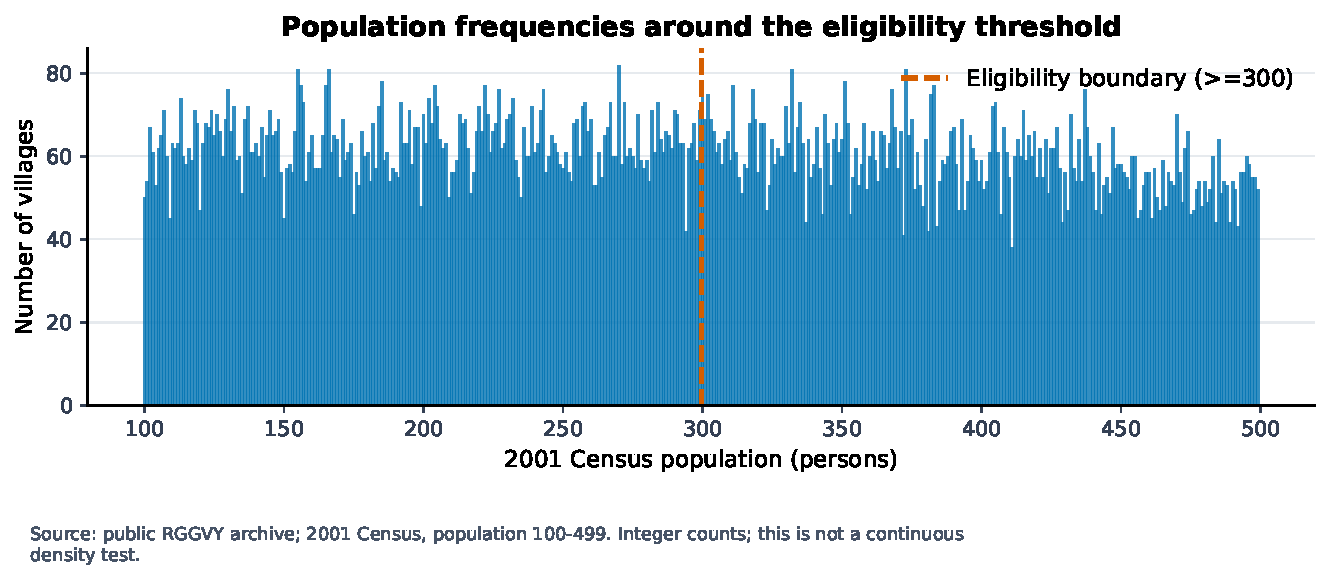
\includegraphics[width=\linewidth,height=3.8in,keepaspectratio]{01_population_frequencies.pdf}
\caption[Population frequencies around the eligibility threshold]{Population frequencies around the eligibility threshold. Source: public RGGVY archive; 2001 Census, population 100-499. Integer counts; this is not a continuous density test.}
\label{fig:gallery01}
\end{figure}
\FloatBarrier
\clearpage
\begin{figure}[!ht]\centering
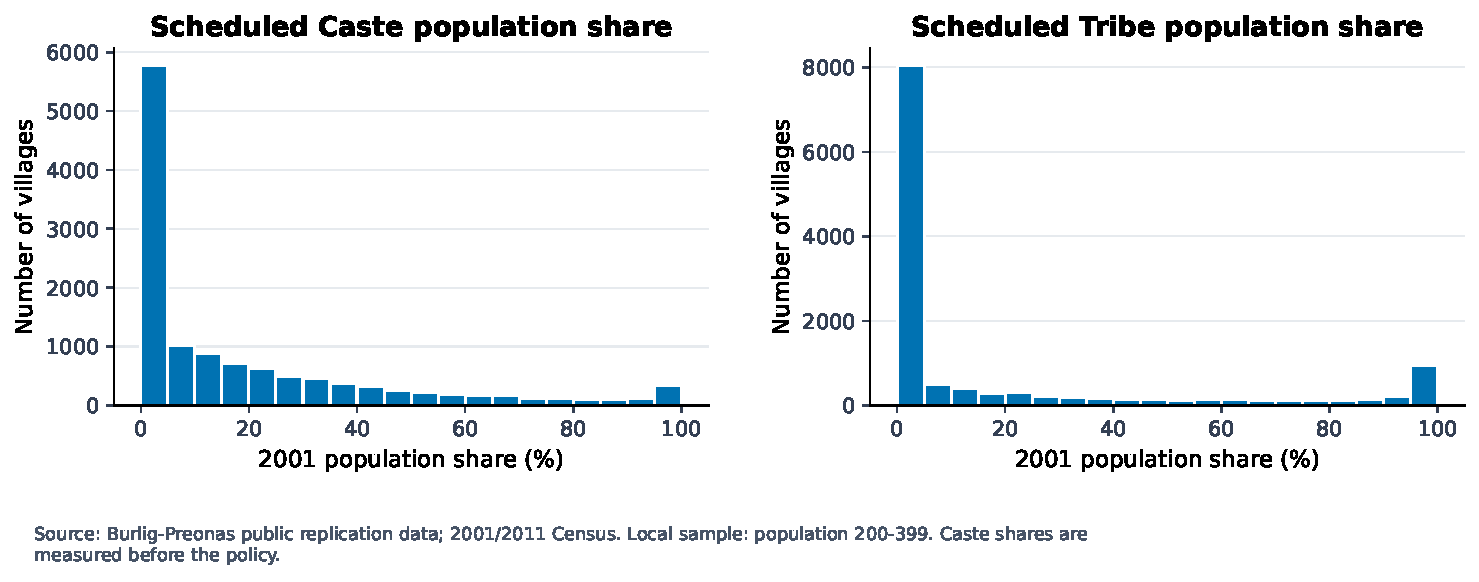
\includegraphics[width=\linewidth,height=5.0in,keepaspectratio]{02_baseline_caste_distributions.pdf}
\caption[Baseline Scheduled Caste and Scheduled Tribe composition]{Baseline Scheduled Caste and Scheduled Tribe composition. Source: Burlig-Preonas public replication data; 2001/2011 Census. Local sample: population 200-399. Caste shares are measured before the policy.}
\label{fig:gallery02}
\end{figure}
\FloatBarrier
\clearpage
\begin{figure}[!ht]\centering
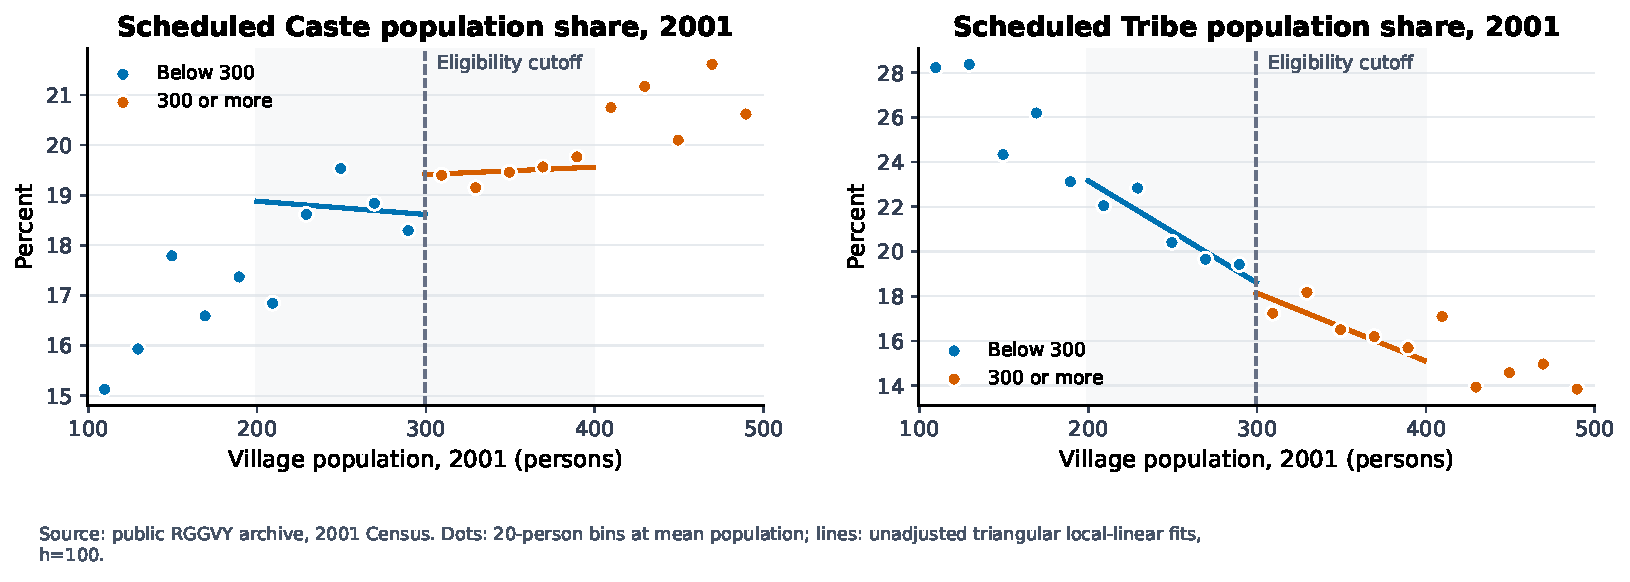
\includegraphics[width=\linewidth,height=5.0in,keepaspectratio]{03_caste_composition_balance.pdf}
\caption[Baseline caste composition at the eligibility boundary]{Baseline caste composition at the eligibility boundary. Source: public RGGVY archive, 2001 Census. Dots: 20-person bins at mean population; lines: unadjusted triangular local-linear fits, h=100.}
\label{fig:gallery03}
\end{figure}
\FloatBarrier
\clearpage
\begin{figure}[!ht]\centering
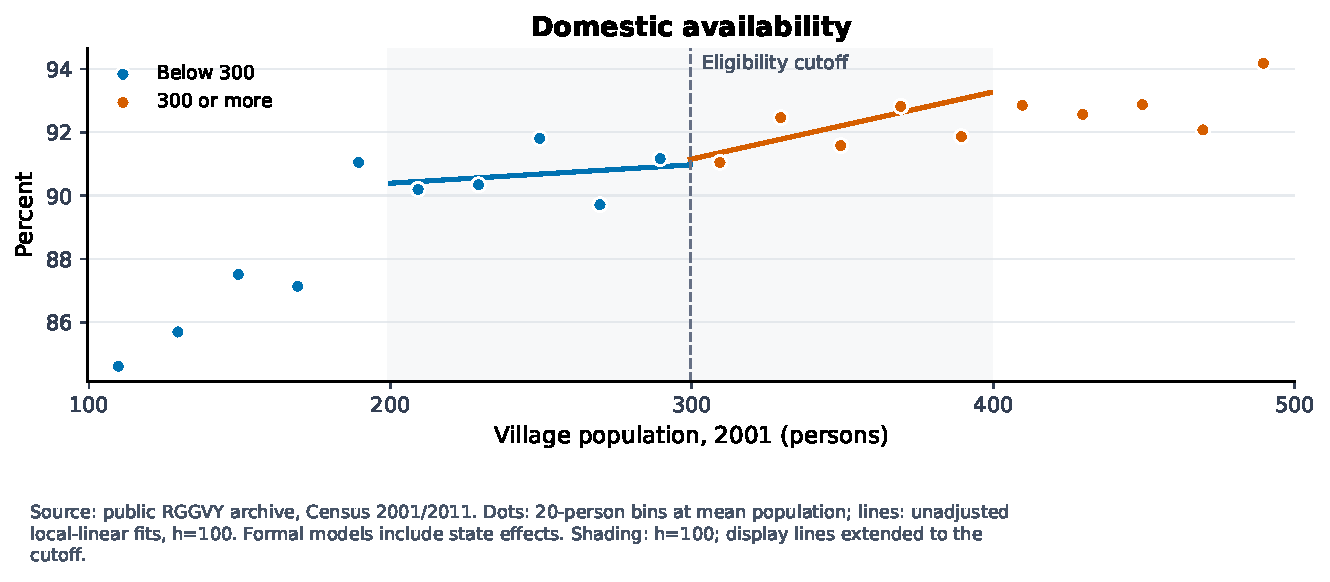
\includegraphics[width=\linewidth,height=5.0in,keepaspectratio]{04_rd_vd_pwr_d_dom_11.pdf}
\caption[Village domestic electricity availability in 2011]{Village domestic electricity availability in 2011. Source: public RGGVY archive, Census 2001/2011. Dots: 20-person bins at mean population; lines: unadjusted local-linear fits, h=100. Formal models include state effects. Shading: h=100; display lines extended to the cutoff.}
\label{fig:gallery04}
\end{figure}
\FloatBarrier
\clearpage
\begin{figure}[!ht]\centering
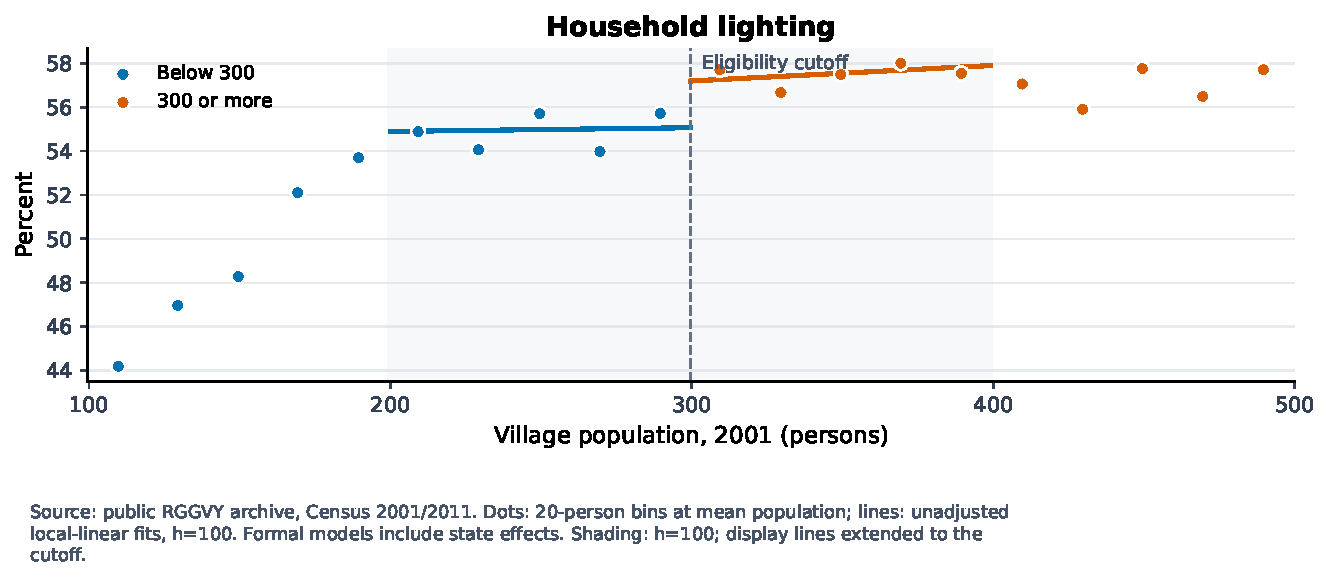
\includegraphics[width=\linewidth,height=5.0in,keepaspectratio]{05_rd_hpca11_msl_elec.pdf}
\caption[Household electric-lighting adoption in 2011]{Household electric-lighting adoption in 2011. Source: public RGGVY archive, Census 2001/2011. Dots: 20-person bins at mean population; lines: unadjusted local-linear fits, h=100. Formal models include state effects. Shading: h=100; display lines extended to the cutoff.}
\label{fig:gallery05}
\end{figure}
\FloatBarrier
\clearpage
\begin{figure}[!ht]\centering
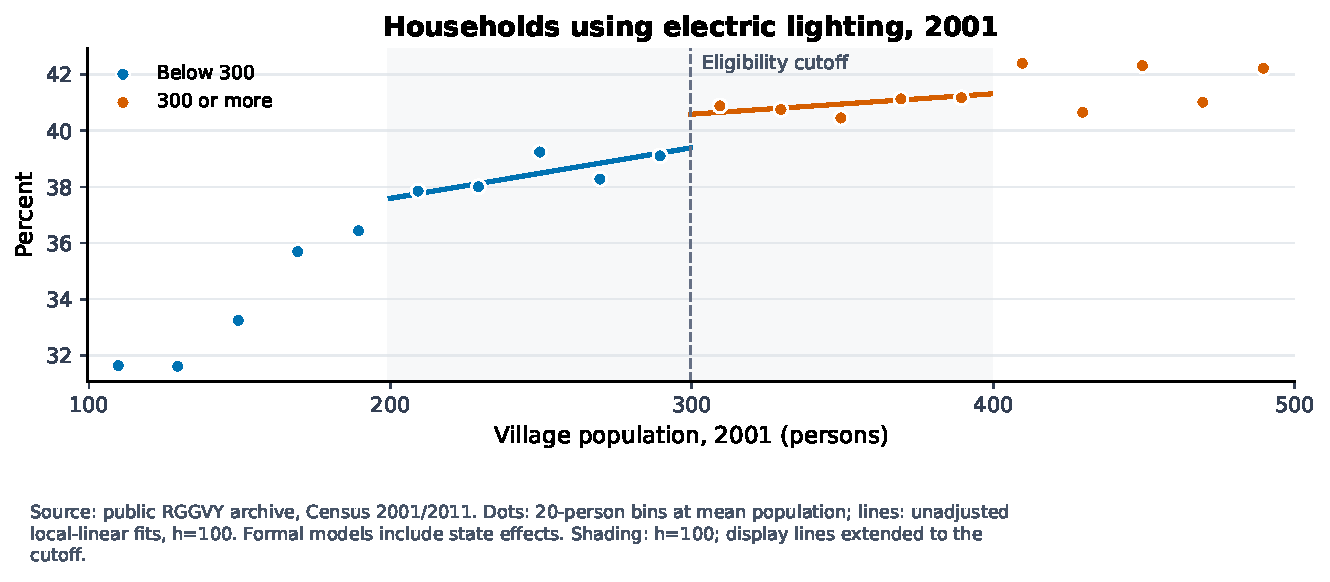
\includegraphics[width=\linewidth,height=5.0in,keepaspectratio]{06_rd_hpca01_msl_elec.pdf}
\caption[Baseline household electric-lighting adoption in 2001]{Baseline household electric-lighting adoption in 2001. Source: public RGGVY archive, Census 2001/2011. Dots: 20-person bins at mean population; lines: unadjusted local-linear fits, h=100. Formal models include state effects. Shading: h=100; display lines extended to the cutoff.}
\label{fig:gallery06}
\end{figure}
\FloatBarrier
\clearpage
\begin{figure}[!ht]\centering
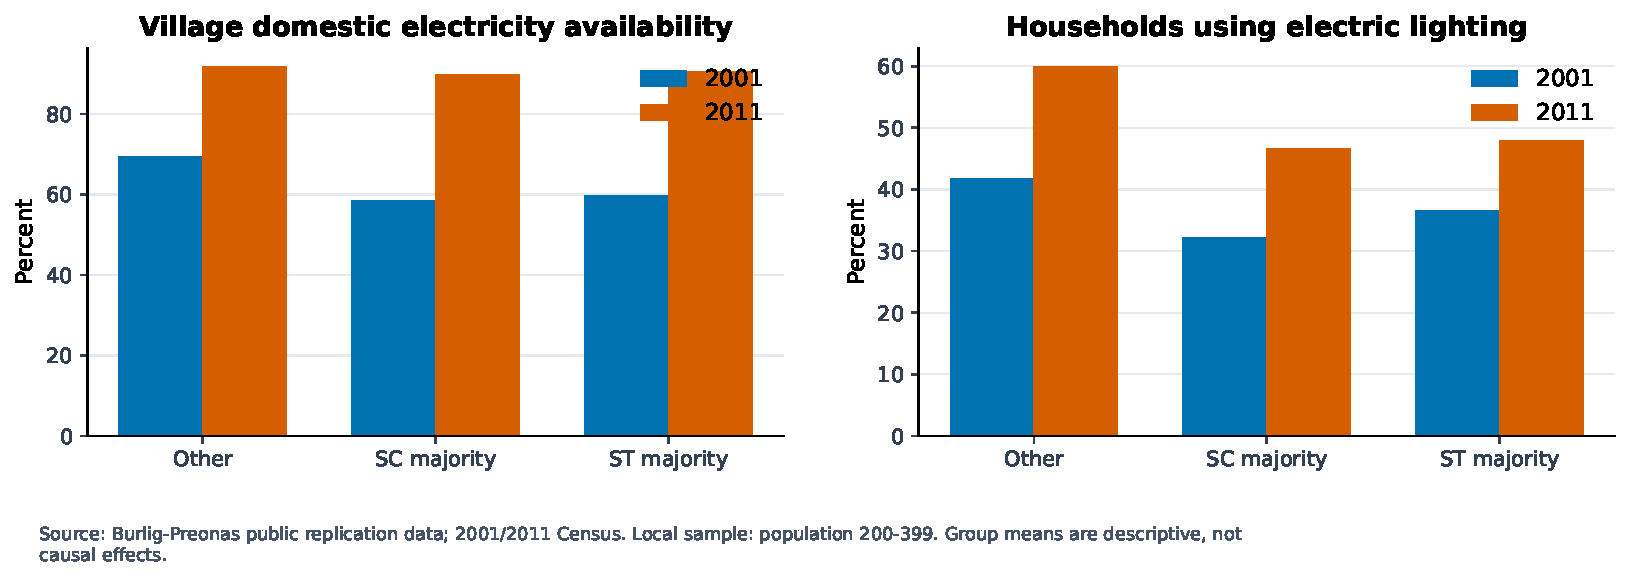
\includegraphics[width=\linewidth,height=5.0in,keepaspectratio]{07_access_and_adoption_by_group.pdf}
\caption[Electricity availability and adoption by composition and year]{Electricity availability and adoption by composition and year. Source: Burlig-Preonas public replication data; 2001/2011 Census. Local sample: population 200-399. Group means are descriptive, not causal effects.}
\label{fig:gallery07}
\end{figure}
\FloatBarrier
\clearpage
\begin{figure}[!ht]\centering
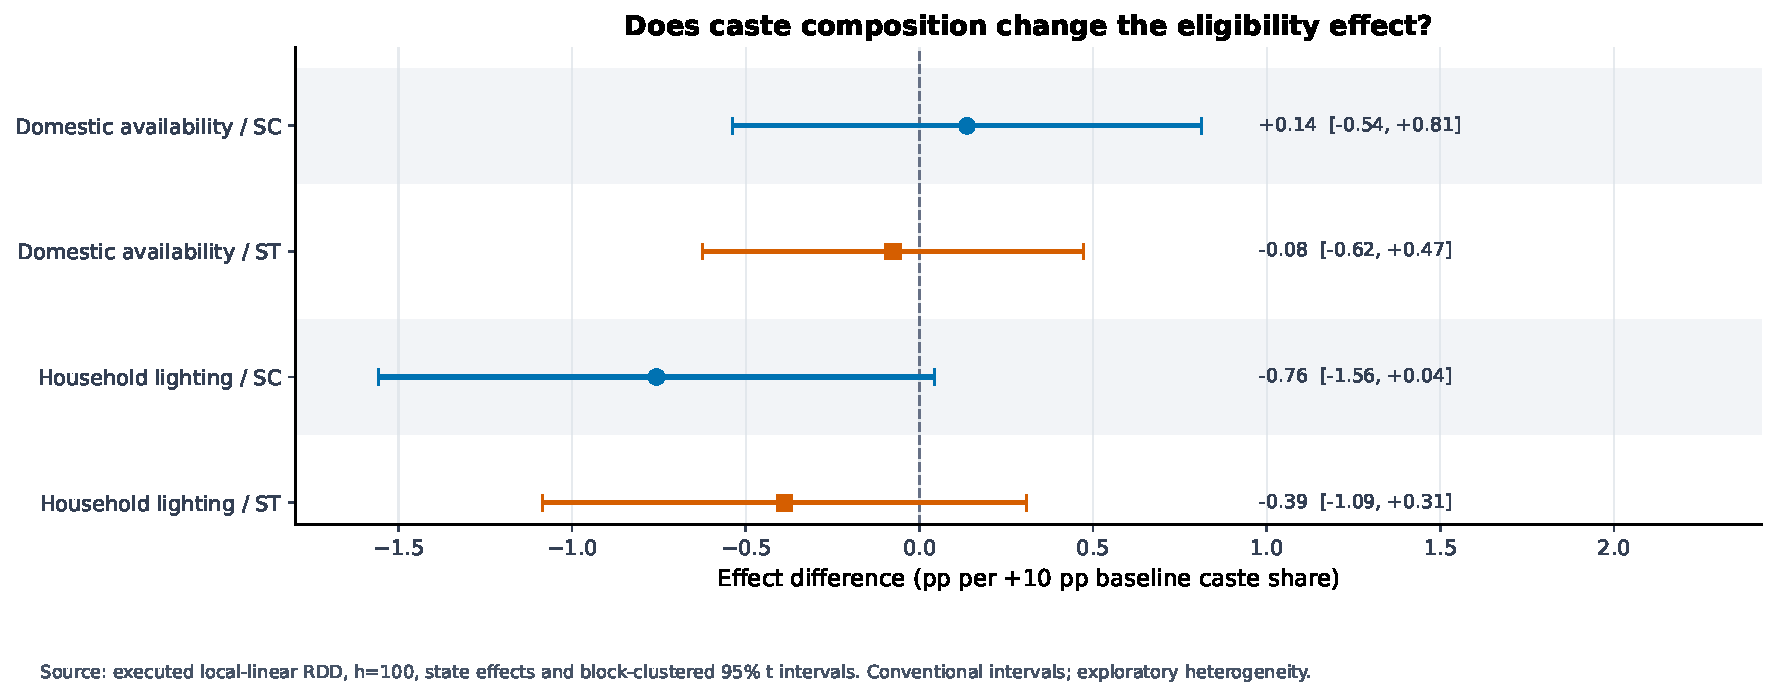
\includegraphics[width=\linewidth,height=5.0in,keepaspectratio]{08_primary_caste_heterogeneity.pdf}
\caption[Primary caste heterogeneity in the eligibility effect]{Primary caste heterogeneity in the eligibility effect. Source: executed local-linear RDD, h=100, state effects and block-clustered 95\% t intervals. Conventional intervals; exploratory heterogeneity.}
\label{fig:gallery08}
\end{figure}
\FloatBarrier
\clearpage
\begin{figure}[!ht]\centering
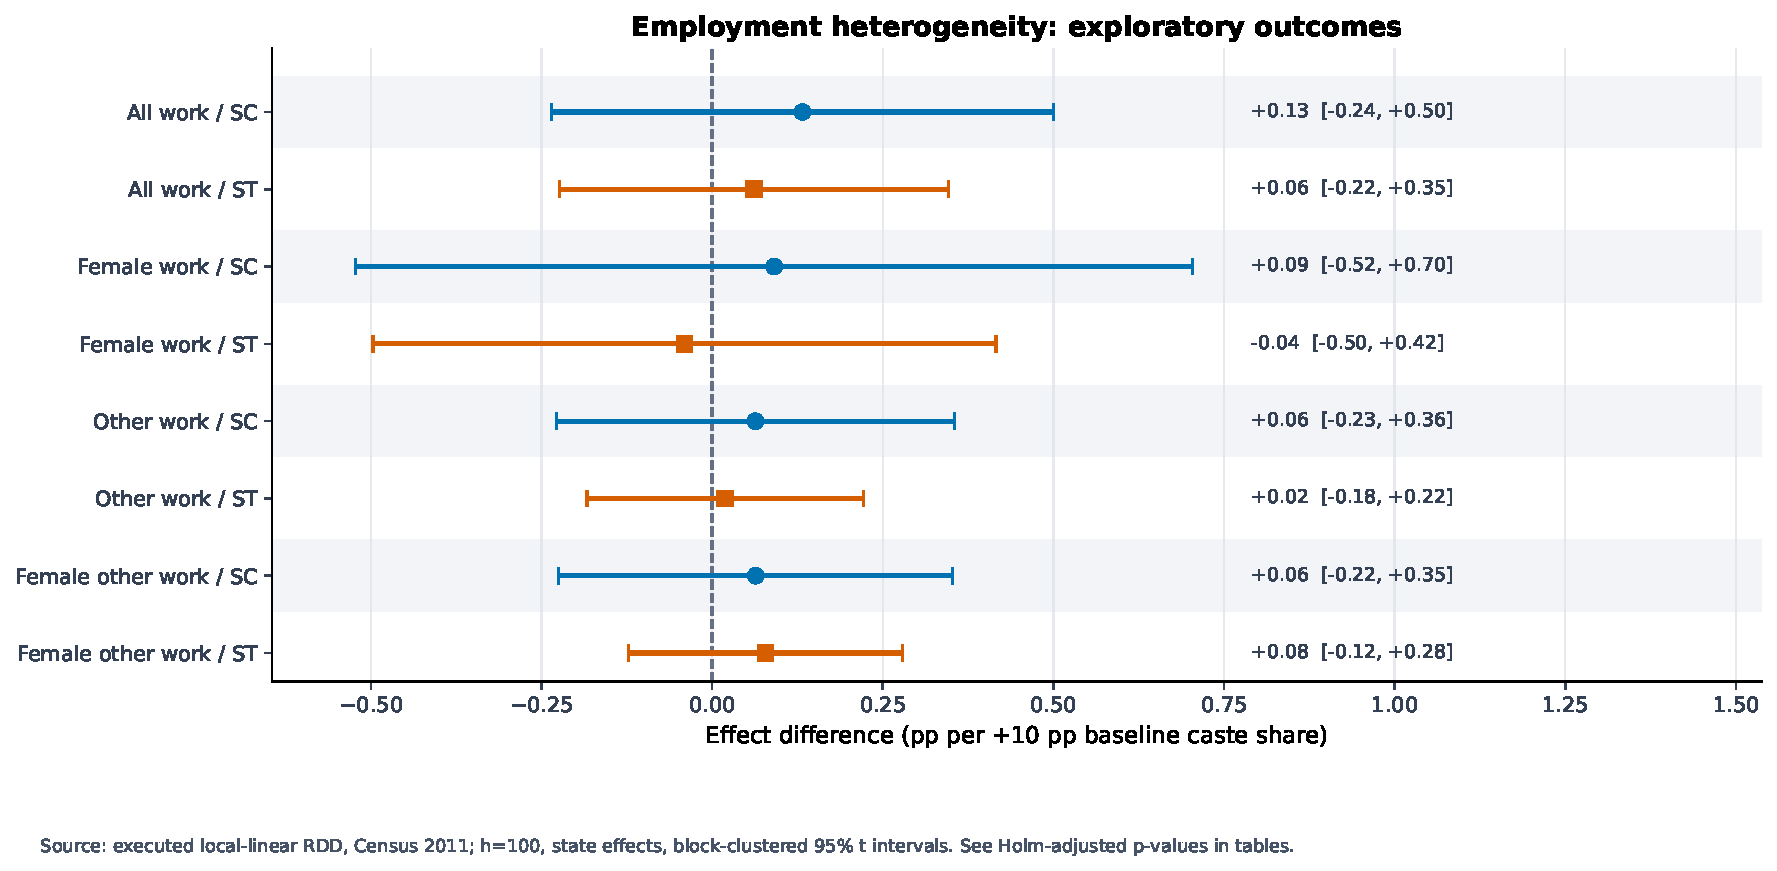
\includegraphics[width=\linewidth,height=5.0in,keepaspectratio]{09_employment_heterogeneity.pdf}
\caption[Exploratory employment-effect heterogeneity]{Exploratory employment-effect heterogeneity. Source: executed local-linear RDD, Census 2011; h=100, state effects, block-clustered 95\% t intervals. See Holm-adjusted p-values in tables.}
\label{fig:gallery09}
\end{figure}
\FloatBarrier
\clearpage
\begin{figure}[!ht]\centering
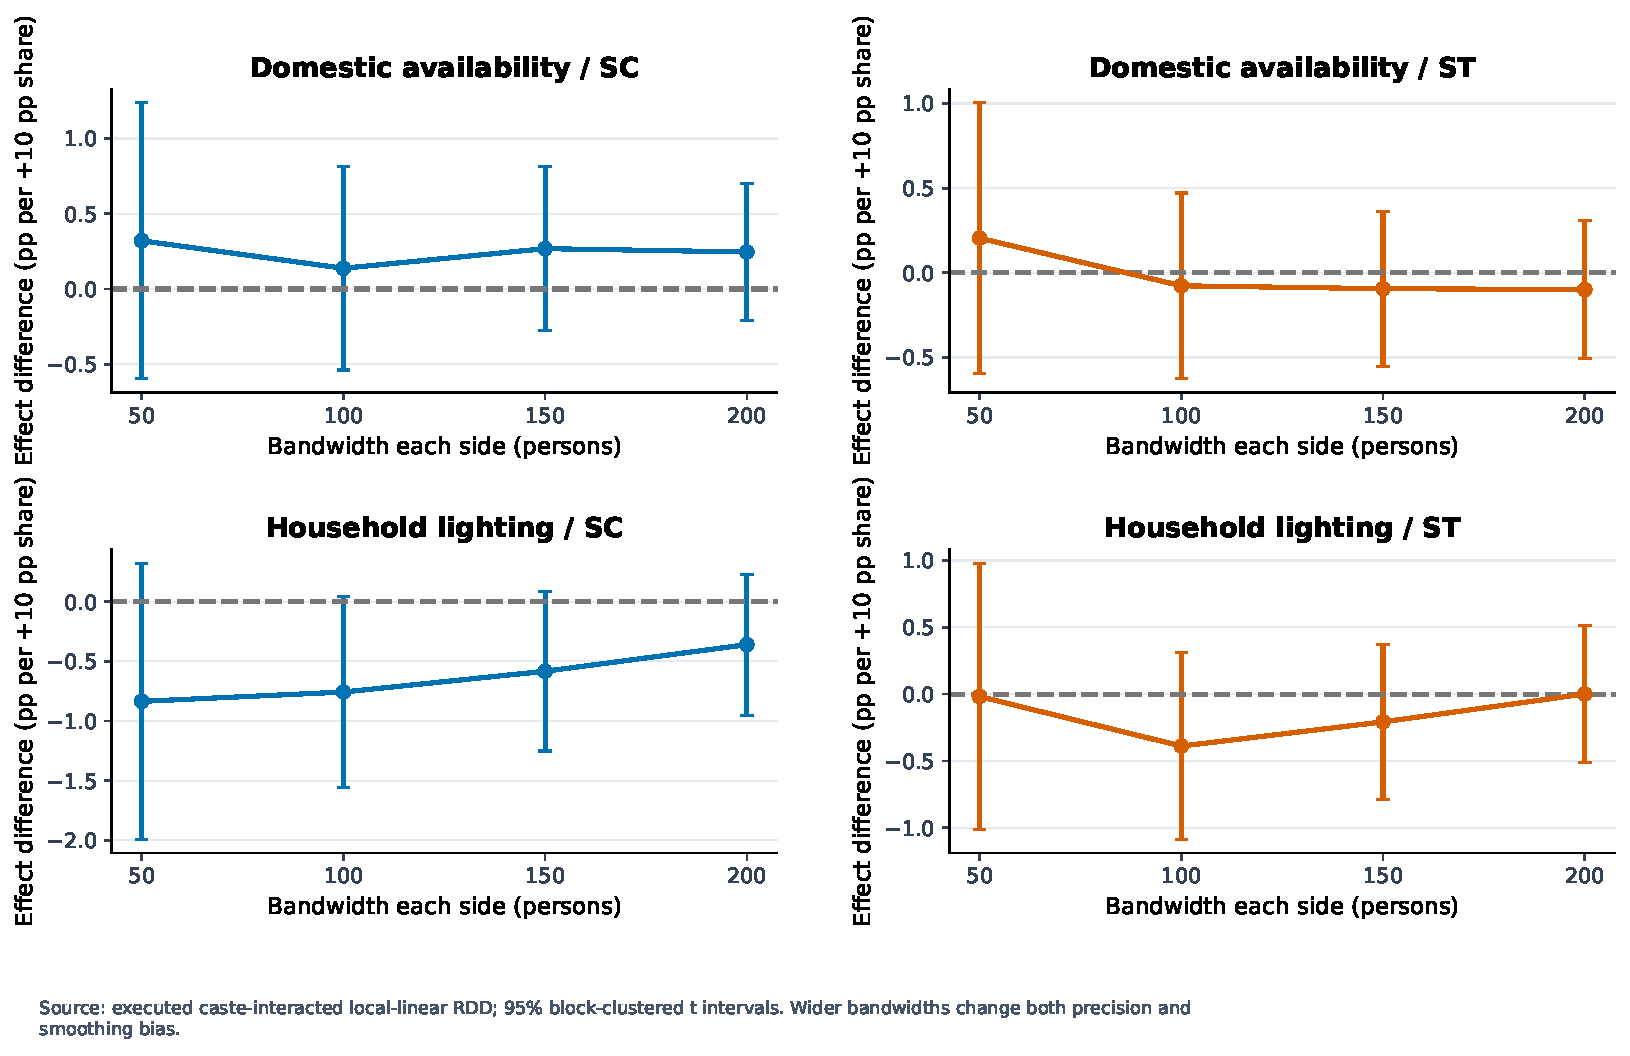
\includegraphics[width=\linewidth,height=5.0in,keepaspectratio]{10_bandwidth_sensitivity.pdf}
\caption[Sensitivity to the population bandwidth]{Sensitivity to the population bandwidth. Source: executed caste-interacted local-linear RDD; 95\% block-clustered t intervals. Wider bandwidths change both precision and smoothing bias.}
\label{fig:gallery10}
\end{figure}
\FloatBarrier
\clearpage
\begin{figure}[!ht]\centering
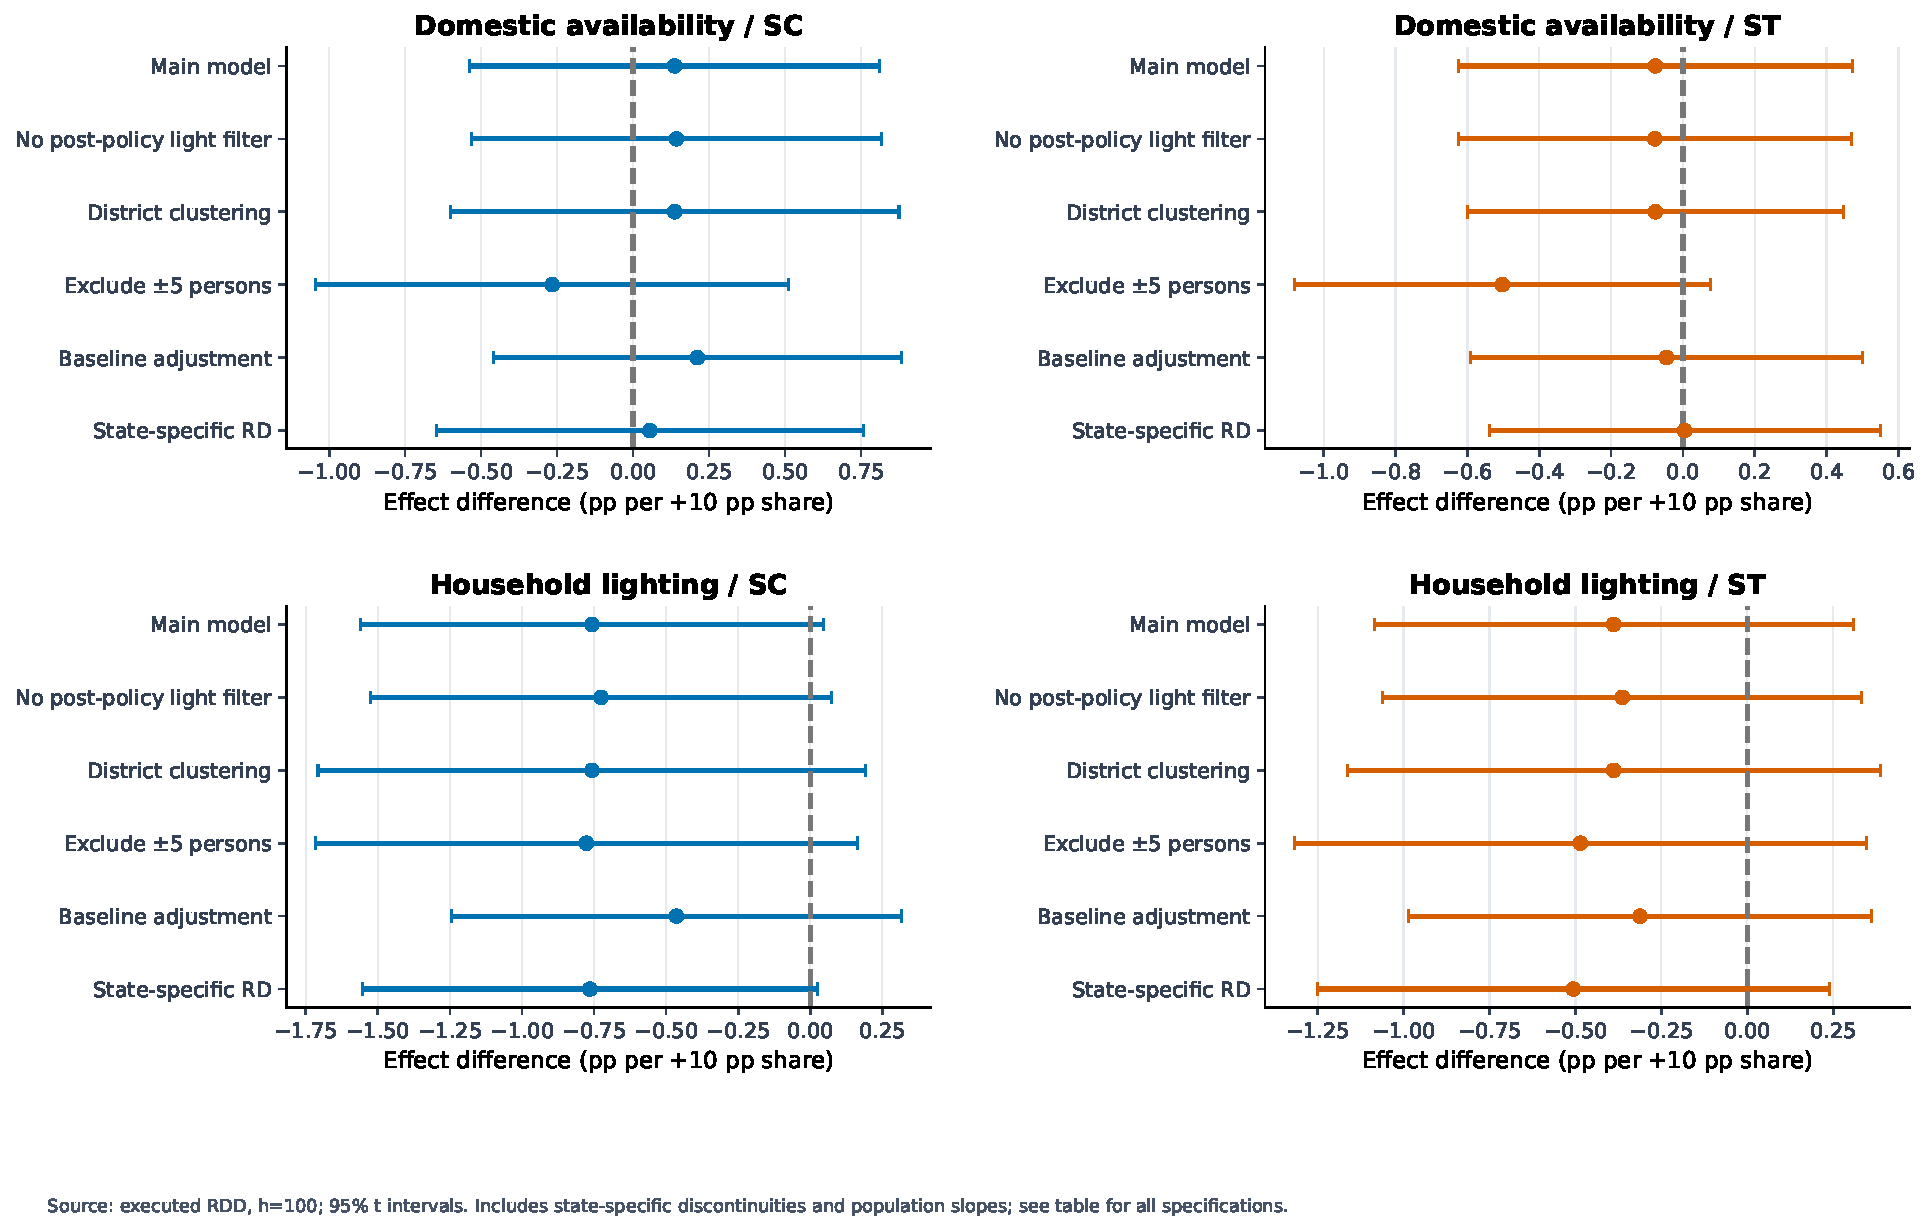
\includegraphics[width=\linewidth,height=5.0in,keepaspectratio]{11_specification_sensitivity.pdf}
\caption[Sensitivity to sample, clustering and regression specifications]{Sensitivity to sample, clustering and regression specifications. Source: executed RDD, h=100; 95\% t intervals. Includes state-specific discontinuities and population slopes; see table for all specifications.}
\label{fig:gallery11}
\end{figure}
\FloatBarrier
\clearpage
\begin{figure}[!ht]\centering
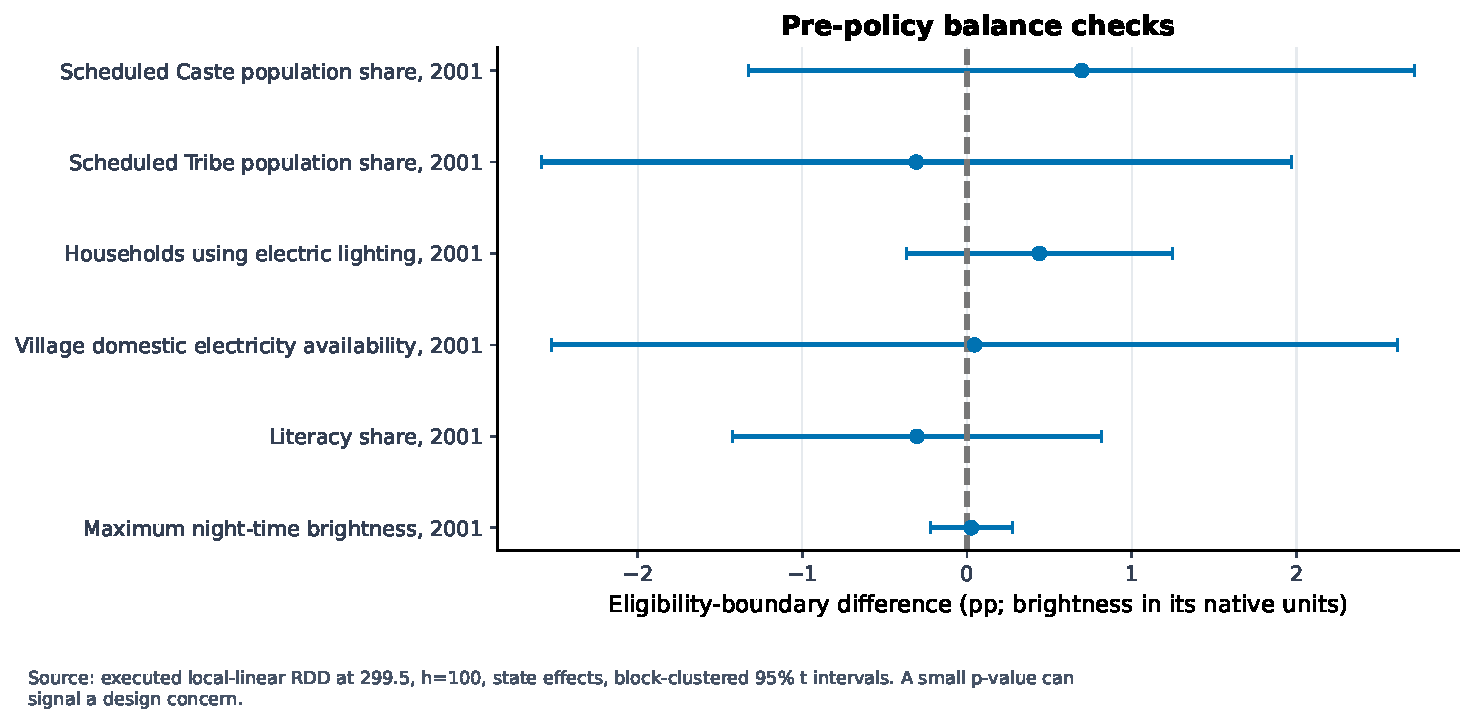
\includegraphics[width=\linewidth,height=5.0in,keepaspectratio]{12_baseline_balance.pdf}
\caption[Predetermined balance at the eligibility boundary]{Predetermined balance at the eligibility boundary. Source: executed local-linear RDD at 299.5, h=100, state effects, block-clustered 95\% t intervals. A small p-value can signal a design concern.}
\label{fig:gallery12}
\end{figure}
\FloatBarrier
\clearpage
\begin{figure}[!ht]\centering
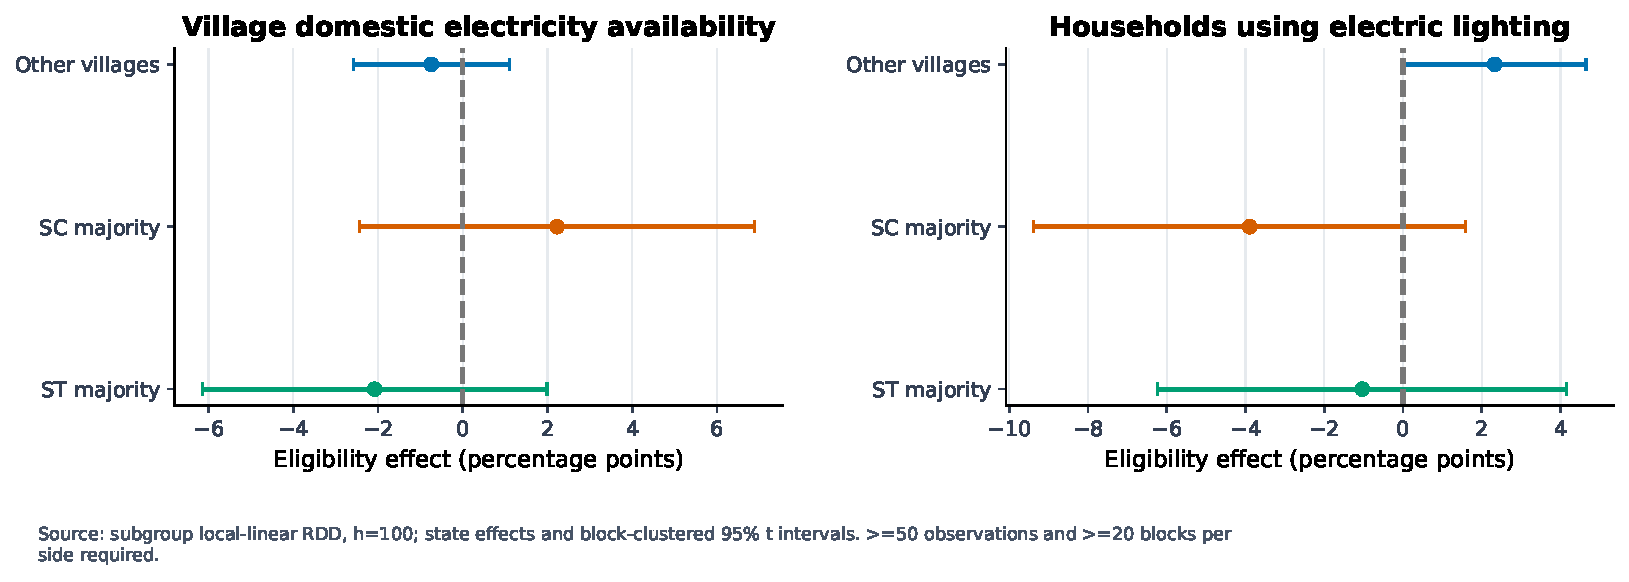
\includegraphics[width=\linewidth,height=5.0in,keepaspectratio]{13_majority_group_rdd.pdf}
\caption[Exploratory eligibility effects by village-composition group]{Exploratory eligibility effects by village-composition group. Source: subgroup local-linear RDD, h=100; state effects and block-clustered 95\% t intervals. $\geq$50 observations and $\geq$20 blocks per side required.}
\label{fig:gallery13}
\end{figure}
\FloatBarrier
\clearpage
\begin{figure}[!ht]\centering
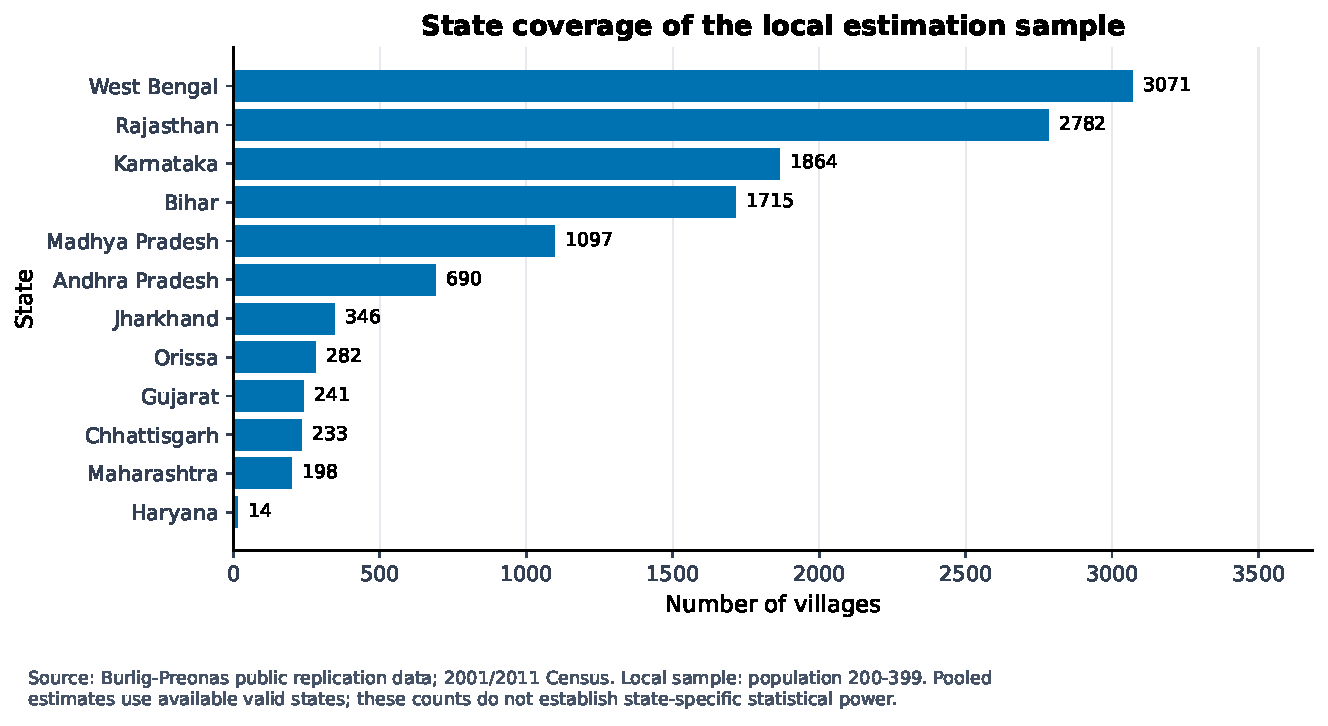
\includegraphics[width=\linewidth,height=5.0in,keepaspectratio]{14_state_sample_coverage.pdf}
\caption[State coverage of the local sample]{State coverage of the local sample. Source: Burlig-Preonas public replication data; 2001/2011 Census. Local sample: population 200-399. Pooled estimates use available valid states; these counts do not establish state-specific statistical power.}
\label{fig:gallery14}
\end{figure}
\FloatBarrier
\clearpage
\begin{figure}[!ht]\centering
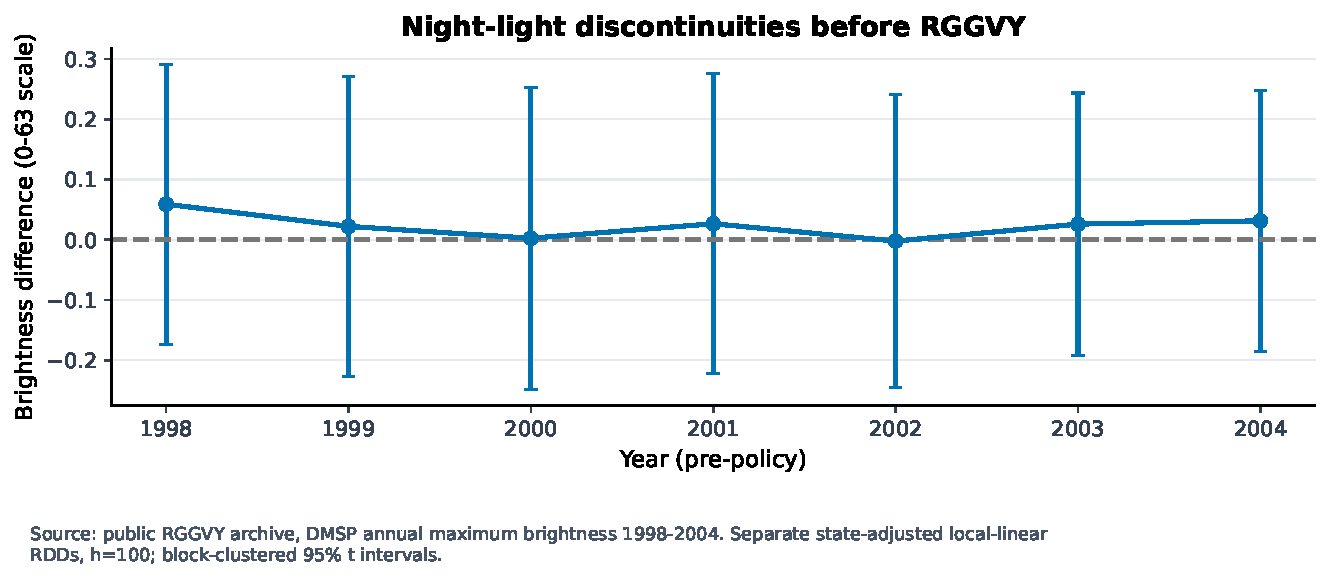
\includegraphics[width=\linewidth,height=5.0in,keepaspectratio]{15_pre_policy_nightlight_checks.pdf}
\caption[Night-light discontinuities before RGGVY]{Night-light discontinuities before RGGVY. Source: public RGGVY archive, DMSP annual maximum brightness 1998-2004. Separate state-adjusted local-linear RDDs, h=100; block-clustered 95\% t intervals.}
\label{fig:gallery15}
\end{figure}
\FloatBarrier
\clearpage
\begin{figure}[!ht]\centering
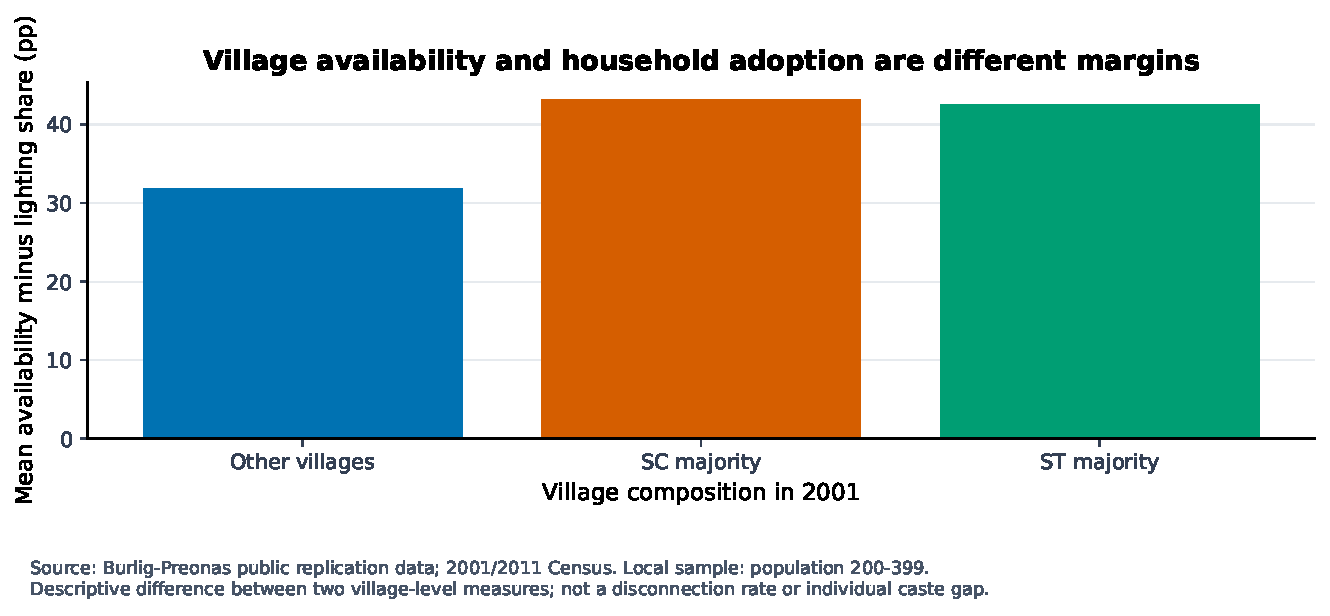
\includegraphics[width=\linewidth,height=5.0in,keepaspectratio]{16_access_adoption_gap.pdf}
\caption[Descriptive gap between village availability and household adoption]{Descriptive gap between village availability and household adoption. Source: Burlig-Preonas public replication data; 2001/2011 Census. Local sample: population 200-399. Descriptive difference between two village-level measures; not a disconnection rate or individual caste gap.}
\label{fig:gallery16}
\end{figure}
\FloatBarrier
\clearpage
\begin{figure}[!ht]\centering
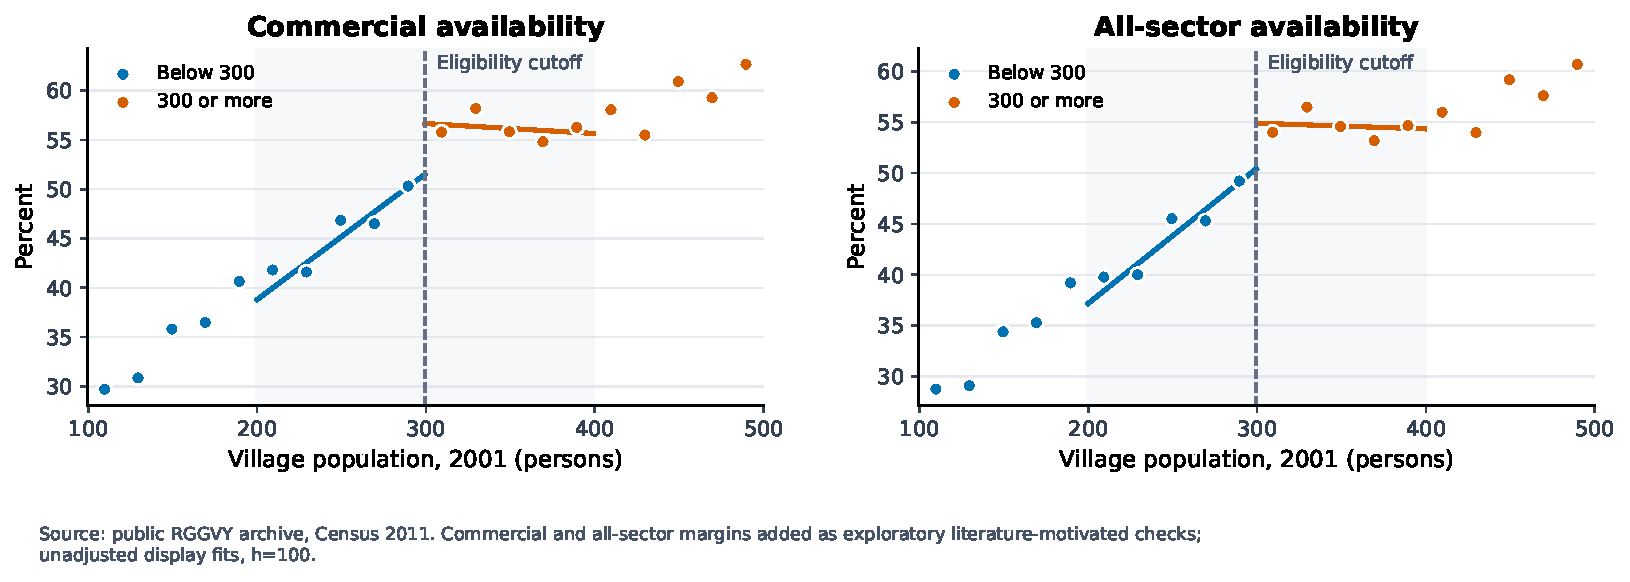
\includegraphics[width=\linewidth,height=5.0in,keepaspectratio]{17_productive_electricity_rdd.pdf}
\caption[Exploratory commercial and all-sector electricity discontinuities]{Exploratory commercial and all-sector electricity discontinuities. Source: public RGGVY archive, Census 2011. Commercial and all-sector margins added as exploratory literature-motivated checks; unadjusted display fits, h=100.}
\label{fig:gallery17}
\end{figure}
\FloatBarrier
\clearpage
\begin{figure}[!ht]\centering
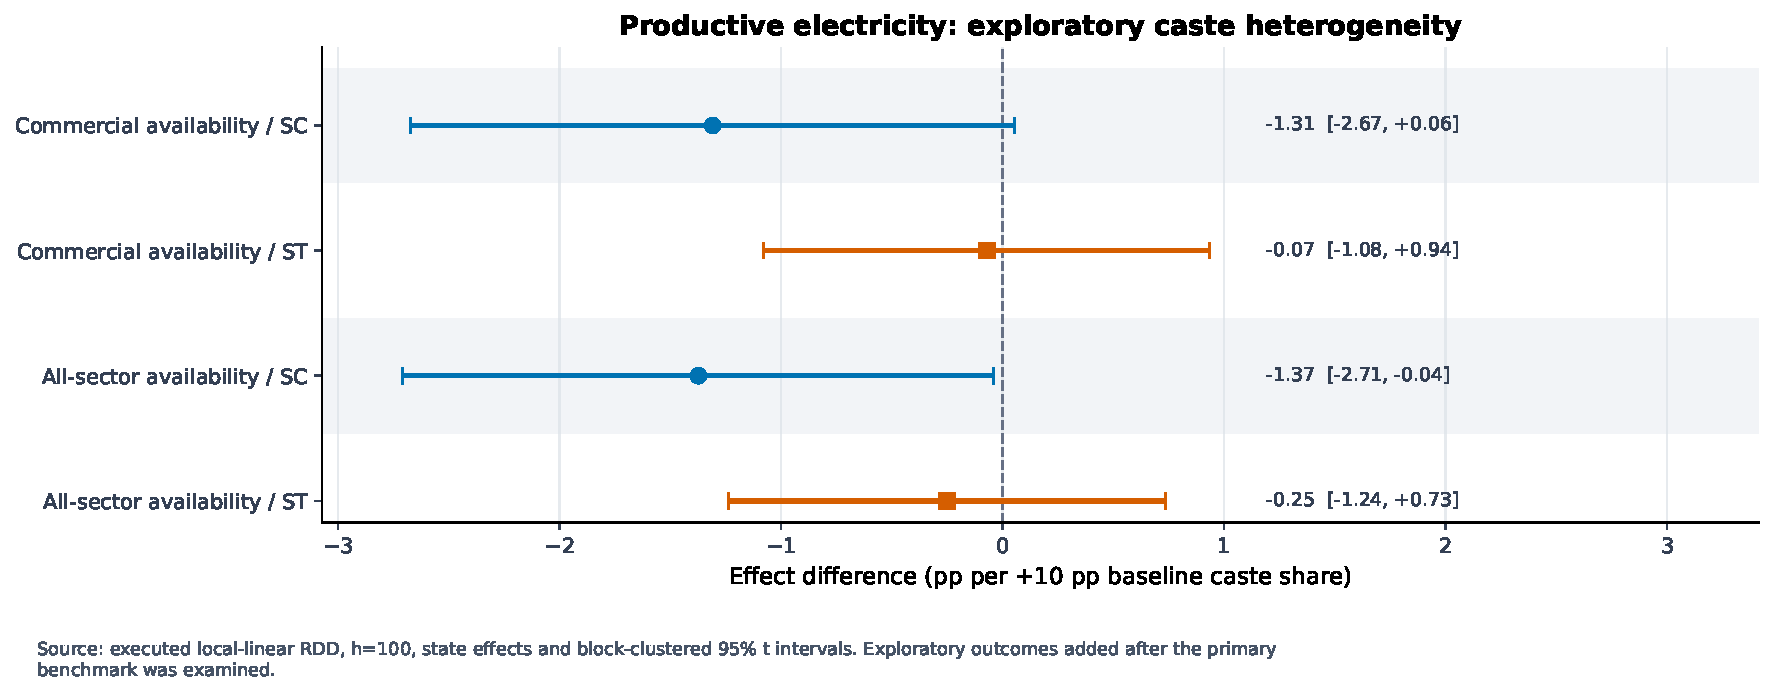
\includegraphics[width=\linewidth,height=5.0in,keepaspectratio]{18_productive_electricity_heterogeneity.pdf}
\caption[Exploratory caste heterogeneity in productive-electricity access]{Exploratory caste heterogeneity in productive-electricity access. Source: executed local-linear RDD, h=100, state effects and block-clustered 95\% t intervals. Exploratory outcomes added after the primary benchmark was examined.}
\label{fig:gallery18}
\end{figure}
\FloatBarrier
\end{landscape}
\clearpage
\end{document}
